\subsection{Overview}
In the last years, the concept of "Software Defined Networking"(SDN) got more and more important. The idea of this concept was created by the introduction of the "OpenFlow" protocol in 2008\cite{Mc2008}. This protocol provides a secure communication between switches of a network and some other part of software. Furthermore the forwarding entries of the routing tables of these switches can be dynamically modified by this protocol. This allows the ability to change network flows at any time to get an optimal behavior for special situations of a network. This is basically the idea of "Software Defined Networking", which is currently promoted and propagated by the "Open Networking Foundation".\footnote{https://www.opennetworking.org/about/onf-overview} 

A Software Defined Network contains basically two important parts. A network with OpenFlow supported switches and a controller. A controller denotes a piece of software which controls at any time the behavior of the network by using OpenFlow. In normal networks each switch is its own controller. When a connection starts the switch makes a lookup in its routing table to forward the packages. If there is no entry it performs some routing algorithm to get this entry. The problem is that there is nothing which has a view on the whole network. For example if a devices has a failure it will take time until each routing device is aware of it. Or maybe if one path of the network is overloaded, it might be faster to send packages via another path. This is a feature, a normal network device can not easily provide. A controller of a Software Defined Network sees the network as graph. It is in a permanent contact with all devices to detect failures. It can get the workload of each switch and can route some communications over other nodes, if a device is overloaded. So the controller can be denoted as the brain of a network and the network nodes as Nerves which follow the orders of the brain. If a new network flow starts, the switch contacts via OpenFlow the controller. The controller decides what to do and sends the switch a flow table entry. A flow table is the routing table in an openflow switch. If the flow finishes the openflow switch deletes this entry from its flow table. So there is never an uncontrolled flow in the network. The concept of a SDN is visualized in picture \ref{sdn}.\\
\begin{figure}[ht]
\centering
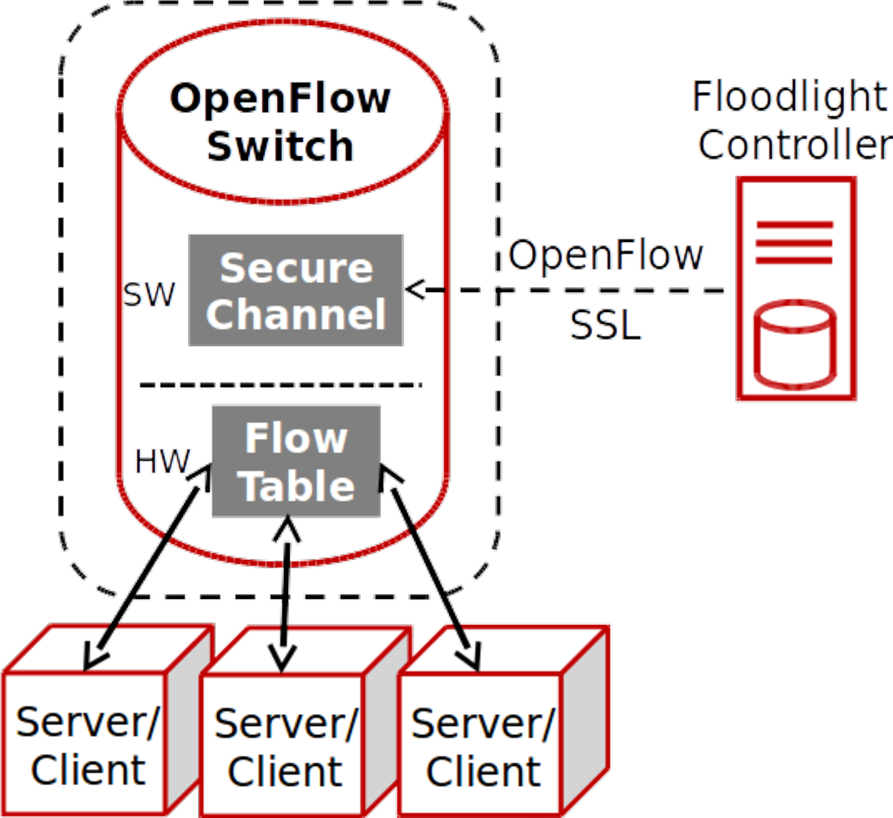
\includegraphics[width=0.25\textwidth]{img/sdn} 
\caption{SDN with Floodlight and Open vSwitch}
\label{sdn}
\end{figure}
 

\subsection{System Setup}
To provide a SDN in the smart Filesystem, the network is organized by the SDN controller Floodlight\cite{flood}. Floodlight is an open source SDN controller, which is written in Java. The fact, that it is written in Java, makes it easy to set it up on many different platforms. Floodlight comes with an OpenFlow implementation for virtual switches as well as physical switches. Moreover it has a lot of additional features. For example features to modify OpenFlow switches or a shortest path routing within a network. Futhermore it is easy to extend Floodlight by using provided interfaces or adding new basic features as so called "Modules". All in all Floodlight allows a quick start in programming a SDN.

As counterpart to the controller, the SDN needs an OpenFlow switch. As told, OpenFlow is a very new protocol. In the moment there are just a few companies, which build switches with OpenFlow support. Besides that, all companies designing these switches for large networks where one is very expensive. A good alternative to this physical switches is the "Open vSwitch" project\footnote{www.openvswitch.org}. With this project it is possible set up a virtual switch with OpenFlow support on a system, which just behaves like a normal switch. This switch can be controlled by Floodlight very easily. A small disadvantage is, that Open vSwitch is currently supporting OpenFlow 1.0(\textbf{CITE!!}), but the latest version is OpenFlow 1.3. However, verion 1.0 supports a lot of features and is, for the needs of the Smart Filesystem sufficient.

This Open vSwitch connects alle parts of the filesystem by using OpenVPN connections and is controlled by Floodlight.     
   
\subsection{Usage in the Smart Filesystem}
In our system we use SDN to overview the flows in the system.   




          